\documentclass[conference]{IEEEtran}

\IEEEoverridecommandlockouts
% The preceding line is only needed to identify funding in the first footnote. If that is unneeded, please comment it out.
\usepackage{cite}
\usepackage{amsmath,amssymb,amsfonts}
%\usepackage{mathtools}
\usepackage{algorithmic}
\usepackage{graphicx}
\usepackage{textcomp}
\usepackage{xcolor}
\def\BibTeX{{\rm B\kern-.05em{\sc i\kern-.025em b}\kern-.08em
    T\kern-.1667em\lower.7ex\hbox{E}\kern-.125emX}}
\begin{document}

\title{Stock market price prediction with Deep Neural Network\\
{\large \textbf{Homework project report}}\\
{\large \textit{Team:} BotosBanda}\\
{\large \textit{Project:} FIN1}
}

\author{\IEEEauthorblockN{Bence Bial}
\IEEEauthorblockA{\textit{Dept. of Automation and Applied} \\
\textit{Informatics}\\
Budapest, Hungary \\
gbenceg@gmail.com}
\and
\IEEEauthorblockN{István Horváth}
\IEEEauthorblockA{\textit{Dept. of Networked Systems} \\
\textit{and Services}\\
Budapest, Hungary\\
histvan1995@gmail.com}
\and
\IEEEauthorblockN{Kristóf Máté}
\IEEEauthorblockA{\
\textit{Dept. of Control for Transportation}\\
\textit{and Vehicle Systems}\\
Budapest, Hungary \\
mate.kry@gmail.com}
}

\maketitle

\begin{abstract}

Stock market price prediction is becoming an important use case of \emph{Deep Neural Network} (\emph{DNN}) nowadays. There is a high expectation of approximating the future values of currency exchanges. However, this is a very difficult task, because sometimes currencies have fluctuating price, which is called volatility. This means that the computer can not simply predict one single value for the future, so there are a lot of challenges to design a useable trading system. Data coming from the markets can be considered as time series, so the developers have to count with the time dependency of the input data. \emph{Recurrent Neural Networks} (\emph{RNN}), including \emph{Long Short-Term Memory} (\emph{LSTM}) can be used for time series prediction tasks. According to the results of existing techniques, \emph{DNN} perform much better compared with other linear forecasting methods.

\end{abstract}

\begin{IEEEkeywords}
Deep Learning, neural network, LSTM, stock market, price prediction, Bitcoin
\end{IEEEkeywords}

\section{Introduction}

\emph{Deep Neural Network} (\emph{DNN}) is an emerging field of Artificial Intelligence. It can be used for multiple types of classification and regression tasks. \emph{DNN} is usually used for solving complex computational problems with huge amount of data, including stock market price prediction. Expectations are getting higher to predict the trends and prices of the foreign exchange market elements. There are a lot of existing techniques for predicting physical assets' price, but cryptocurrencies cause critical issues in forecasting methods. This makes really hard to fulfill the requirements.

Forecasting algorithms can be divided into two main categories: linear (\emph{AR}, \emph{MA}, \emph{ARIMA}, \emph{ARMA}) and non-linear models (\emph{ARCH}, \emph{GARCH}, \emph{Neural Network}) \cite{b6} \cite{b7}. The non-linear models (including \emph{DNN}) brought such a good improvement to the prediction results that researchers have to deal with it.

In this article we present a data processing method and a system based on \emph{DNN} that can predict the price of a stock market element (BTC to USDT). This is a time series analysis task, for which we use a regression model. According to the scholarly literature, the best way to accomplish the task is using \emph{LSTM} components in the network. We consider Bitcoin to USDT exchange dataset as training dataset for one year interval. We downloaded this dataset from Poloniex.

\subsection{Cryptocurrencies}

Bitcoin (BTC) is the most popular cryptocurrency nowadays \cite{bitcoin}. It is a decentralized digital currency that enables instant payments to anyone, anywhere in the world. Bitcoin uses peer-to-peer technology (called Blockchain) to operate with no central authority: transaction management and money issuance are carried out collectively by the network. Therefore, Bitcoin has got strongly volatile price, so it is hard to forecast the future value.

Tether (USDT) is a Blockchain-based cryptocurrency which's cryptocoins are backed by an equivalent amount of traditional fiat currencies, for example USD.

\subsection{LSTM}

\emph{Long Short-Term Memory} (\emph{LSTM}) is usually used for time series data modelling \cite{lstm}. \emph{LSTM} is a recurrent component, that can handle time dependence \cite{rnn}. It has got an internal memory cell, which provides weights for old and new input data.

\subsection{Existing techniques}

Cryptocurrencies have strongly volatile stock market price in contrary with other exchanges. Consequently, it is really hard to achieve accurate prediction for future values. Prediction and analysis of stock market data have got an important role in today’s economy. According to this, there are researchers who would like to a much better result in this kind of tasks.

\cite{b2} applies multivariate \emph{k-Nearest-Neighbour} (\emph{kNN}) regression model for financial time series forecasting. In their approach the nearest neighbors that bear referential information for a target time series are identified by exploiting the financial correlation from the historical data.

In \cite{b4} fully connected neural networks were tested for predicting FOREX market values.

\cite{b1} uses \emph{LSTM} network for Bitcoin price prediction. They took the closing price of Bitcoin in USD from the Coindesk Bitcoin Price Index as input features. They used CRISP data mining methodology and they achieved classification accuracy of 52\% and a RMSE of 8\%.

\cite{b3} article presents a deep learning framework for financial time series using a deep learning-based forecasting scheme that integrates the architecture of stacked autoencoders and \emph{LSTM} to generate the deep and invariant features for one-step-ahead stock price prediction.

In \cite{b5} \emph{Convolutional Neural Network} (\emph{CNN}) was used for predicting the stock price of a company based on the historical prices available. They used day-wise closing price of two different stock markets, National Stock Exchange (NSE) of India and New York Stock Exchange (NYSE). They compared their results with ARIMA model and it has been observed that the neural networks are outperforming the existing linear model (ARIMA).

\cite{b0} article presents a deep learning model predicting the stock price movement followed by a financial model which places orders in the market. The model is based on the dataset consists of tick by tick candlesticks. They propose a way of modeling the high frequency trading problem using Deep Neural Networks.

\section{Data acquisition and preparation}

\subsection{Data sources}

In the time series forecasting task, we would like to predict the price of Bitcoin in USDT. So we collected BTC to USDT exchange values from Poloniex. In addition to this we gathered BTC to ETH, BTC to XRP, BTC to LTC, BTC to XMR and BTC to DASH exchanges' weighted averages. The downloaded data contains candlesticks' OHLC values and the volume. The period of one candlestick is 300s.

According to the scholarly literature, we engineered our features as following. The main essential feature is the weighted average of the price of exchange. Furthermore, we also took the stock value as an input feature.

\vspace{3px}

\begin{itemize}
  \item Bitcoin candlestick OHLC values: open, high, low, close
  \item Volume
  \item BTC to ETH, BTC to XRP, BTC to LTC, BTC to XMR and BTC to DASH weighted averages
\end{itemize}

\vspace{3px}

We have already tried to add SMA, EMA and RSI indicators to the input feature set, but this approach resulted incorrect operation. The network could predict more precisely when omitting these items.

\subsection{Data splitting}

There are 10 features for the training, but we only need the weighted average of BTC to USDT as predicted output. We need to divide the dataset into training, cross validation and test sets to get the best performance out of the network. Initially we used the following dataset division for the learning process (Figure \ref{fig:TrainTestSplit}).

\begin{itemize}
  \item Train - 70\%
  \item Cross validation - 20\%
  \item Test - 10\%
\end{itemize}

\begin{figure}
  \centering
  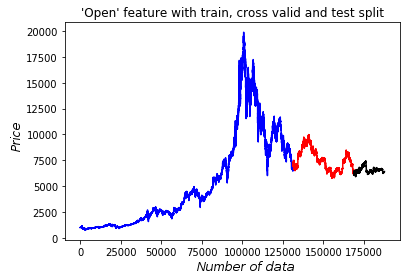
\includegraphics[width=80mm, keepaspectratio]{figures/train_test_split_1.png}
  \caption{Train-test split}
  \label{fig:TrainTestSplit}
\end{figure}

The dataset we have is relatively big, so we decided to increase training set and decrease cross validation set, because smaller sized validation set was just enough. The modfification of data splitting also  improved prediction accuracy a bit.

\begin{itemize}
  \item Train - 80\%
  \item Cross validation - 10\%
  \item Test - 10\%
\end{itemize}

\subsection{Data scaling}

We put an emphasis on data preprocessing during the development. Bitcoin's price can be considered as a very specific time series, so we had to handle it in a specific way. In contrary with physical currencies, Bitcoin is not being supervised by a central bank, so the volatility is very high.

Our research in scholarly literature shows that various scaling methods used in previous time series prediction systems. In our work we also tried to find the best way for preprocessing the data to get the more better results. We tried 4 different scaling method on our time series.

\textbf{Case 1} - \emph{Scale the whole dataset in standard way}. This method performed poorly, because the minimum and maximum value of the observed period was in a large range ([1000, 20000]) and the majority of scaled data got scaled to a relatively small range (using StandardScaler: [-1, 1]). In this case validation error was low, but the error measured in the training set was hundred times greater. We have soon realized, that this method is unusable for the current task.

\textbf{Case 2} - \emph{Scaling in windows}. We have tried different scaling window sizes. Applying the configuration with the size of 2500 performed the best, but there was no significant difference compared with the values in range 1000-5000. We dropped all the training data where the range of a training example intersected with 2 windows to avoid large jumps in data that would misleaded the training process. This method resulted a useable scaling.

\textbf{Case 3} - In the previous method we fitted our scaler on the training set and scaled the whole validation and test set with that last scaler. This made the prediction to convergate to the same value, so all predictions were pointing upwards or downwards ignoring all input data. So we decided to fit our first scaler on the data in first window, then scale the data in the first window and the next window. After scaling the next window, we can train our data on those original values as we are not using information from future. Consequently, we can also scale validation and test set with their own scaler. This way our prediction on real charts looked much better as predictions were not pointing always the same way.

\textbf{Case 4} - In previous method even if we used MinMaxScaler, the data were approximately in range of -4 to 4, for example when the price was going up all the way in the window and was smaller in the previous window which we trained the scaler on. Consequently, we decided to scale the data after the train-validation-test division. Separate scaler was used on every example. For example if we were making predictions from previous 250 candles of chart, then a scaler was fitted on those 250 data (X) and were transformed with this scaler. Then transformed the result value (y) with the same scaler. So in case of a MinMaxScaler, all values in X were between 0 and 1, and the y value could be only a slightly over 1 or under 0. This scaling method also does not use information from the future as we already know all X values when we are predicting y. This method' performance is proved to be the best.

\begin{figure*}[!ht]
  \centering
  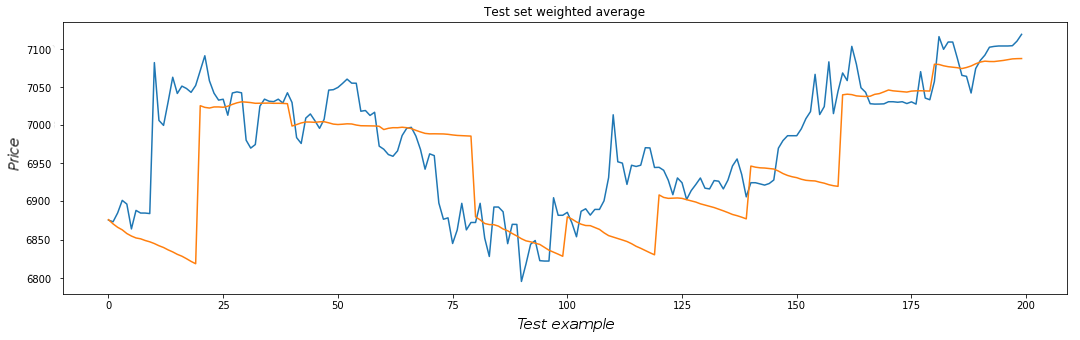
\includegraphics[width=170mm, keepaspectratio]{figures/test_pred_1.png}
  \caption{Test prediction with model 1}
  \label{fig:TestPred1}
\end{figure*}

\subsection{Autoencoder}

We have already tried autoencoder network for removing noise from time series. This method producted a smooth function of OHLC data which we considered as an additional feature for our network. However, the results got worse after the expansion of the input features. This is probably because of the cryptocurrencies' volatility. If we filter the high frequency alteration from the input data, the network will not learn this important feature. Consequently, we omitted this input feature in the later phase of the development.

\section{Implementation}

As framework, we used Keras with Tensorflow backend. The computing unit was a PC with I7-4930k CPU and a Nvidia GTX1070 8GB GPU.

% 1st milestone
\subsection{Model 1}

The first model composititon included only fully connected layers, as shown below.

\vspace{3px}

\begin{itemize}
  \item \textit{Fully connected layer:} 200 neurons, activation: sigmoid
  \item \textit{Fully connected layer:} 100 neurons, activation: sigmoid
  \item \textit{Fully connected layer:} 100 neurons, activation: sigmoid
  \item \textit{Output layer:} 1 neuron, activation: sigmoid
\end{itemize}

\vspace{3px}

We used mean squared error as loss function and the Adam optimizer algorithm. Moreover, we trained the data in 2500 epochs and we also used early stopping with the patience of 20 epochs. Early stopping shut down learning at the 125th epoch. We found out, that it is a really bad model, because we found out that the network did not learn appropriately during the whole training process. Consequently, we need needed to add layers that can handle the time dependece of our data. We need a Recurrent Neural Network (RNN).

\begin{figure}[!ht]
  \centering
  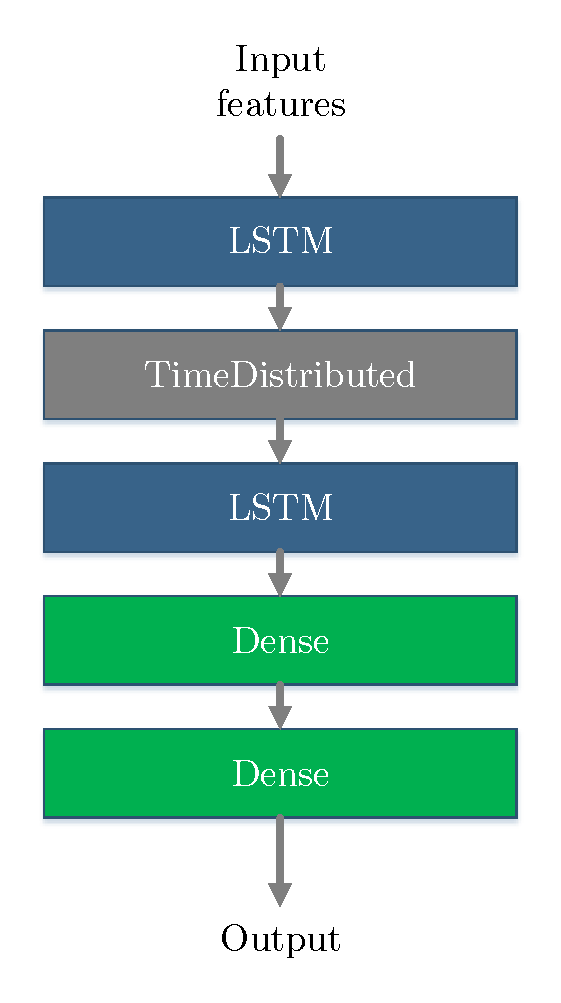
\includegraphics[width=40mm, keepaspectratio]{figures/nn-model-3.pdf}
  \caption{Model 3 architecture}
  \label{fig:nn-model-3}
\end{figure}

% 2nd milestone
\subsection{Model 2}

Referring to the results of the previous model architecture, we added Convolutional and \emph{LSTM} layers to the network. The configuration was the following:

\vspace{3px}

\begin{itemize}
  \item \textit{1D Convolution layer:} 64@5, activation: ReLU
  \item \textit{1D MaxPooling layer:} pool size: 2, strides: 2
  \item \textit{1D Convolution layer:} 32@3, activation: ReLU
  \item \textit{1D MaxPooling layer:} pool size: 2, strides: 2
  \item \textit{LSTM layer:} 64 cells
  \item \textit{Output layer:} 1 neuron, activation: sigmoid
\end{itemize}

\vspace{3px}

Figure \ref{fig:TestPred2} shows the predictions for our second model. We can consider a substantial improvement compared to the first one, but it is still not good enough.

\begin{figure*}[!ht]
  \centering
  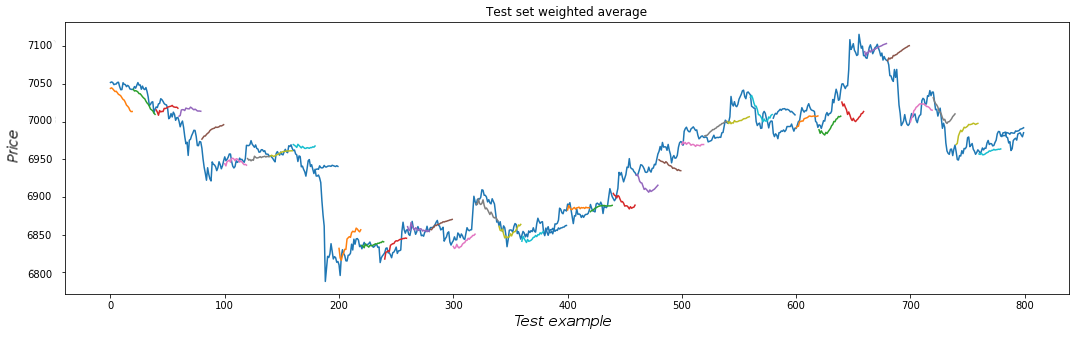
\includegraphics[width=170mm, keepaspectratio]{figures/test_pred_2.png}
  \caption{Test prediction with model 2}
  \label{fig:TestPred2}
\end{figure*}

After this model's prediction we concluded that convolutional layers does not fit to our task appropriately. Maybe this is because of the volatile property of the cryptocurrency values.

% The last model
\subsection{Model 3}

Our last models structure is shown below:

\vspace{3px}

\begin{itemize}
  \item \textit{LSTM layer:} 128 cells, with return sequences
  \item \textit{TimeDistributed layer:} 10 neurons
  \item \textit{LSTM layer:} 128 cells
  \item \textit{Fully connected layer:} 128 neurons, activation: ReLU
  \item \textit{Output layer:} 10 neurons, activation: linear
\end{itemize}

\vspace{3px}

The third model shows the best performance so far. We added two \emph{LSTM} layers with 128 neurons, that can handle the time series' time dependence. We also added a \emph{TimeDistributed} layer with 10 neurons which improved the result, too. At the top of the network there is a fully connected layer with 128 neurons, which is followed by the output layer. We predict the current value of all the input features for one time step. Figure \ref{fig:TestPred3} illustrates the predicitons of the third model. As it can be seen, the prediction can catch the trends of the price movement at almost every prediction step. Moreover the chart shows that the predicted price tries to fit the target value, e.g. near the 5230th and 5480th test example.

\begin{figure*}[!ht]
  \centering
  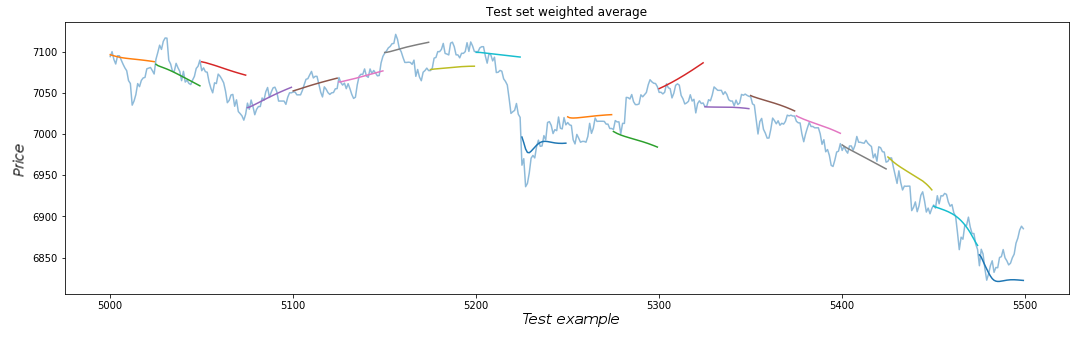
\includegraphics[width=170mm, keepaspectratio]{figures/test_pred_3.png}
  \caption{Test prediction with model 3}
  \label{fig:TestPred3}
\end{figure*}

\subsection{Types of training}
\label{TypesOfTraining}

In the first case predict one candlestick data from the previous 250 candlesticks. Then we put the predicted data to the input of the network, so we predict from the data we already predicted. This method can be considered as a sliding window, that has an overlapping with a number of 249 and includes the immediate predecessor of the current data. This method is demonstrated in \ref{eq_train_data_1}, where $k$ is the current time step, $n$ is the number of the features, $l$ is the lookback, $X^k$ is the current input feature set, $X^k_i$ is the i\textsuperscript{th} column of $X^k$ and $y^k$ is the current output vector. In our case $n=10$ and $l=250$.

\begin{equation}
\label{eq_train_data_1}
  \begin{gathered}
    X^k = \begin{bmatrix} X_{2}^{k-1} & X_{3}^{k-1} & \cdots & X_{l}^{k-1} & y^{k-1} \end{bmatrix} \\[5mm]
    X^k \in \mathbb{R}^{n\times l} \qquad
    y^k \in \mathbb{R}^{n\times 1}
  \end{gathered}
\end{equation}

In another case, we tried to predict only the weighted average of 5, 10 or 15 candlesticks. In this case the dimension of output was only 3. However, this method did not give a good predictions for the Bitcoin's price.

\section{Conclusion}

We started from a very simple model structure and continuously updated the model. As expected, adding \emph{LSTM} layers resulted the most significant change in usability as they are designed to find complex interrelations in time series.

Another idea was to use one-dimensional convolutional layers to recognize some pattern in data. According to our experimentation, the train and validation error decreased a bit. However, this decreasing did not mean that our model performed better on real problems. The real problem is to predict prices in a longer term or at least some time steps as only 1 step is not enough to recognize the trend of the market. A solution to this problem would be an error function optimizing for longer forecasts and not just 1 timestep.

The network's forecast (prediction for 25-50 timesteps) often looked like a random guess, so the model was probably underfitting. Adding more features decreased the loss almost every time, but did not fix the usability issue of the model. The model was always making prediction upwards or downwards. As usability we consider the forecast that could be used by a trader.

We ended up adding OHLC and volume data from bitcoin and the weighted averages from another 5 famous coins (ETH, XRP, LTC, XMR, DASH). Correlation between these coins improved the model but adding all of their features (e.g. OHLC) would be too many variables to predict each timestep and the error would be very large.

\section{Future works}

There are a plenty of opportunities in research and develop our approach. We could use classification model as classifying the direction of the trend of the chart. In this case we could define an arbitrary number of classes (e.g. -10\%, -5\%, +5\%, +10\%) and predict the ratio of increment or reduction.

Another idea is to use Reinforcement Learning system to test our model in real-time trading. This would be a real and practical use case of our system.

Moreover we could find the optimal value of the hyperparameters using \emph{Hyperas} software package.

Furthermore, we could add different kind of features to the system. For example the main actions of the blockchain system. Traders have a direct emotional effect on this feature, so maybe this could improve the predicted results.


\section{Summary}

In this article we presented a Deep Neural Network system, which's goal is to forecast Bitcoin to USDT exchange price. We did some research in relevant scholarly literature and described existing techniques and the main concepts of this field. Then we demonstrated our data acquisition and the data preprocessing. We put an emphasis te decision on data splitting and scaling. We tried different ways to solve this problem and we engineered the input features according to this.

In the beginning we used only fully connected layers for training, but this method led to a definitely poor result. Fotinately, we have already found this fact out in the early stage of the development process. Consequently, we absolutely agree with the fact described in relevant scholarly literature, that we needed to use Long Short-term Memory components. \emph{LSTM} components imply more complex computations, on account of the more complex internal structure.

Then we described two other models later. Our last model structure performed the best. Finally we concluded our work and we did some recommendations for possible future works.

\vspace{20px}

\begin{thebibliography}{00}

\bibitem{b6} Asteriou, Dimitrios and Hall, Stephen, ``ARIMA Models and the Box-Jenkins Methodology'', 2016

\bibitem{b7} Engle, Robert F., ``Autoregressive Conditional Heteroscedasticity with Estimates of the Variance of United Kingdom Inflation'', Econometrica, vol. 50, no. 4, 1982, pp. 987--1007.

\bibitem{bitcoin} Satoshi Nakamoto, ``Bitcoin: A Peer-to-Peer Electronic Cash System'', 2009

\bibitem{lstm} Sepp Hochreiter, Jürgen Schmidhuber, ``Long Short-Term Memory'', Neural Computation, pp. 1735-1780, 1997

\bibitem{rnn} Pushparaja Murugan, ``Learning The Sequential Temporal Information with Recurrent Neural Networks'', 2018, arXiv:1807.02857

\bibitem{b2} T. Ban, R. Zhang, s. Pang, A. Sarrafzadeh and D. Inoue, ``Referential kNN Regression for Financial Time Series Forecasting'', 2013, pp. 601--608.

\bibitem{b4} Jirí Vahala, ``Prediction of Financial Markets Using Deep Learning'', Bachelor's Thesis, Masaryk University Faculty of Informatics, 2016

\bibitem{b1} S. McNally, J. Roche and S. Caton, ``Predicting the Price of Bitcoin Using Machine Learning'', 2018 26th Euromicro International Conference on Parallel, Distributed and Network-based Processing (PDP), Cambridge, 2018, pp. 339--343.

\bibitem{b3} Bao W, Yue J and Rao Y, ``A deep learning framework for financial time series using stacked autoencoders and long-short term memory'', PLOS ONE 12(7): e0180944, 2017

\bibitem{b5} Hiransha M, Gopalakrishnan E.A., Vijay Krishna Menon, Soman K.P., ``NSE Stock Market Prediction Using Deep-Learning Models'', Procedia Computer Science, Volume 132, 2018, pp. 1351--1362

\bibitem{b0} Prakhar Ganesh, Puneet Rakheja, ``Deep Neural Networks in High Frequency Trading'', 2018, arXiv:1809.01506

\end{thebibliography}

\end{document}
